\documentclass{article}
\usepackage{amsmath}
\usepackage{amsfonts}
\usepackage{amsthm}
\usepackage{graphicx} % Required for inserting images
\usepackage[
backend=biber,
style=ieee,
]{biblatex}
\addbibresource{ref.bib} %Import the bibliography file
\usepackage[a4paper, total={6in, 10in}]{geometry}
\usepackage{hyperref}
\title{Training a self driving vehicle with formally verifiable reinforcement learning}
\author{Anthony Marchiafava, Jober't Aladwan, Sara Basili}
\date{May 16 2023}

\begin{document}

\maketitle
%\newpage
%\tableofcontents
%\newpage

\section{Motivation}
% * How to convince others your work is worthwhile?
Reinforcement learning (RL) is a powerful technique used to solve some world tasks in which an agent learns by interacting with an environment. The agent learns a policy that dictates which action should be taken when in various states. However, the agent's interactions often begin without any knowledge of the environment and must learn an optimal policy by getting rewards from these interactions. If a self-driving car designed to learn to drive on the street instead learns to use off-street paths, it must be trained further to prevent such actions and get closer to the optimal on street driving policy. As this more optimal policy develops, can this policy have some assurance that the off-street behavior would not return? Can this policy incorporate other constraints such as stopping at stoplights? Can anything be said to assure someone that these unacceptable actions will not take place?


\section{Challenges}
% problems which will arise, this is more the specific challenges the motivation gives rise to so this needs to be rewritten.
\paragraph{Finding an optimal policy.} Reinforcement learning uses rewards to develop an optimal policy. These rewards are designed to encourage actions which lead to more desired states and discourage actions which lead to less desirable states. However, this can have unintended consequences where a less than ideal action is encouraged before a better action is discovered. An agent designed to drive through a racetrack may learn to drive off-course if it leads to fast results and there are no constraints to discourage that behavior. Properly building rewards to only encourage optimal behavior will be paramount in creating this safety-oriented agent.
\paragraph{Modeling the environment.} When assessing the value of an algorithm which has learned some actions on its own, the quality of the environment from which the agent gets its state is very important. If the agent is supposed to learn to not drive off a racetrack, there must be some non-racetrack area in which it can be penalized for entering. When learning in an artificial simulation, a more closely related real environment and simulated environment would lead to more realistic policies.


\section{Related Work}
% * Short history of reinforcement learning
% to show how other people solved similar challenges and what is your inspiration TODO:Write up some of the other papers on RL for continuous action spaces, other learning techniques such as imitation learning, and move many of the citations from Motivation paragraph down here. 
Different formal verification techniques for Reinforcement Learning have been used in a variety of contexts such as self driving cars \cite{https://doi.org/10.48550/arxiv.1904.07189}, human resource management \cite{10.1145/3577204}, multi-agent systems \cite{9357415}, trajectory generation \cite{9287929}, and could apply to many other problems. These techniques intend to improve the quality of the reinforced learning by incorporating domain knowledge \cite{https://doi.org/10.48550/arxiv.1801.08099}, show the ability to reach certain states \cite{9357415}, and show safety \cite{9724872}. These and other similar problems have been solved using popular techniques such as Neural Fitted Q Iteration \cite{10.1007/11564096_32}, Deep Q-Learning \cite{https://doi.org/10.48550/arxiv.1801.08099} and Deep Deterministic Policy Gradient (DDPG) \cite{https://doi.org/10.48550/arxiv.1509.02971}. The process for building Linear Temporal Logic is based on \cite{10.1007/978-3-319-41540-6_17}.

\section{Objectives}
% * We want our agent learn how to complete the track without violating its constraints 
% narrow down the goal to show exactly what challenges you want to address specifically. What is the goal?
Our work will show that some formally defined constraints can be incorporated into a reinforcement learning agent based on Linear Temporal Logic in a manner similar to \cite{https://doi.org/10.48550/arxiv.1801.08099}\cite{https://doi.org/10.48550/arxiv.1904.07189}. With some modifications, a reinforcement learning (RL) algorithm may include domain knowledge which the agent would not otherwise start with and dramatically decrease the need to explore actions whose consequences are already known to be unacceptable. This agent will manage a self-driving wheeled vehicle in a racetrack like environment, and its goal will be to drive through the racetrack while not entering the goal region on a red light and not going off-track.

\section{Problem formulation}
%talk about the problem and express it using technical definitions precisely and mathematically so this needs a complete rewrite.
We can express this problem as a Markov decision process (MDP). MDPs are sequential decision problem for a fully observable, stochastic environment, with a transition model which only requires the current state and an action to get to the next state, and a subsequent reward that gets our agent closer to some goal \cite{russel2010}. The MDP consists of a set of states, a set of actions in each state, a transition model which takes an action and the current state which are used to provide the next state, and a reward function. These are all used to generate a policy which provides an action which should be taken given a state. This policy should provide, for any state encountered, an action which will get the agent closer to our goal.

To win the game the agent must finish the track (by getting into the goal region) without going off the road. The agent will not enter the goal region on a red light. Formally expressed with Linear Temporal Logic our problem is to optimize a policy for an agent constrained by the following:
\begin{equation}
    \square ( \text{goal} \implies \square \text{goal}) \wedge \square ( \text{unsafe} \implies \square \text{unsafe} ) \wedge \diamond \text{goal}
\end{equation}

Our goal, then, is to find some optimal policy $\pi^{*} : S \rightarrow A$, such that the policy will provide an optimal action for each state.

Our problem is broken down into a MDP made up of the state of the environment, modeled with CoppeliaSIM, and an actor in the simulator. This actor interacts with the environment and our actions will be based on fulfilling the logical criteria expressed in (1). This logical criteria is converted to a Limit-Deterministic Büchi Automata (LDBA). The LDBA is then used to label the current state of the program so we are aware of the safe or unsafe states. If the car goes off the boundaries of the track or enters the goal region while the light is red, we consider that unsafe.

We used two methods for learning an optimal policy, Neural Fitted Q-Learning and Deep Deterministic Policy Gradient. These both rely on the idea of a Q-function and a policy. The Q-function is an optimal action-value function. Provided some state and action, our Q-function provides us the value of doing that action in that state \cite{russel2010}.
\begin{equation}
    Q(s,a) = R(s) + \gamma \sum_{s'} P(s' | s,a) \max_{a'} Q(s', a')
\end{equation}
Where $Q(s,a)$ is the Q-function of some state $s$ and some action $a$, $R(s)$ is the reward function which specifies the reward for a given state ($s$), $\gamma$ is a discount factor to discount the value future rewards, and we would sum up the transition model ($P(s'|s,a)$) which shows the probability of reaching the next state $s'$ from state $s$ doing action $a$ which is chosen, and $Q(s',a')$ shows the utility value of action ($a'$) from state ($s'$) which is the expected reward. This would require a transition model, but it is possible to learn without such a model. For Q-learning we could instead use \cite{10.1007/11564096_32}:

\begin{equation}
    Q(s,a) \leftarrow Q(s,a) + \alpha(R(s) + \gamma \max_{a'} Q(s',a') - Q(s,a))
\end{equation}

So if we keep a table of our utility values from our state action pairs and update this table until we sufficiently explore the search space. Then we can use the Q table to discover which action to take for an optimal policy without needing the transition model. This can work for modeling discrete actions and discrete states, but proves challenging with problems with continuous action spaces and continuous state spaces.

\section{Methodology}
%briefly explain what methods you expect you will use
For our task of testing logically constrained learning, we created a working version of a Markov Decision Process contained within CoppeliaSim to act as the environment and adopted the framework as seen in \cite{hasanbeig2022lcrl} to create our logical constrained learning simulations.The knowledge of the environment each agent will have will be composed of its X and Y velocity, the status of the traffic light, and how far the agent is in from the goal object. Our environment would be converted to a discrete state space for the agents which are configured to only work with a discrete space, and left continuous for the agents that were capable. Our agent could choose to go north, east, south, west, northeast, southeast, northwest, southwest, or remain stationary. Our agent would have its goal region marked on the street, and a light which would change color. The main job would be to get into the goal region while the light was not marked red, while not hitting any of the sides of the street. Entering the goal region while the light was red or hitting the sides of the street were specified as unsafe states, being in the goal region while the light was green was the accepting goal state. We chose three methods of generating a policy to explore: Basic Q-Learning, Neural Fitted Q-Learning (NFQ), and Deep Deterministic Policy Gradient (DDPG).

\begin{figure}
    \centering
    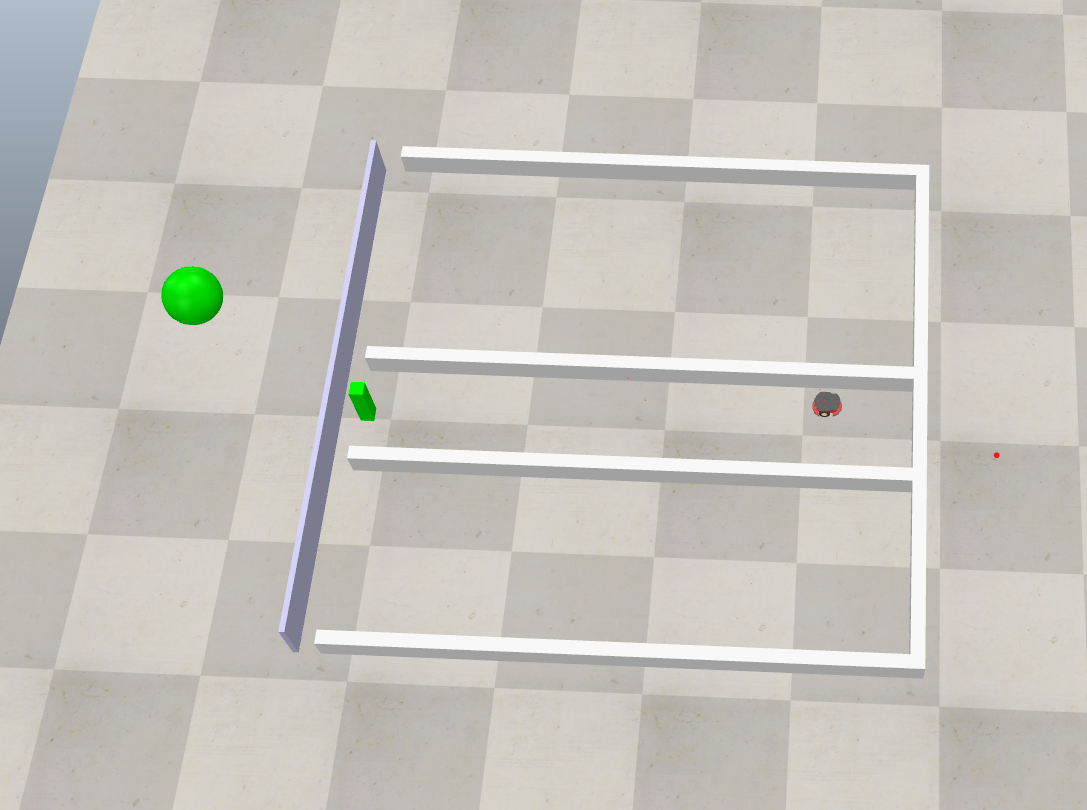
\includegraphics[keepaspectratio,scale=0.5]{media/track.png}
    \caption{Simulation Track in CoppeliaSim}
    \label{track}
\end{figure}
\paragraph{Neural Fitted Q-Learning}
This algorithm allows offline learning of Q-values with a densely connected neural network. Instead of storing a complete Q-table of every state and action from that state, we instead could use a neural network to represent the value function. We would generate a large table of experiences made up of the current state $s$, the action taken $a$, and the next state $s'$ from having an agent interact with the simulated environment. Then we would use a multi-layer perceptron (MLP) with two layers to train on the entire sample set, so that it could approximate Q values.

\paragraph{Deep Deterministic Policy Gradient}
%explain DDPG. Briefly.
This algorithm is based on the actor-critic approach to allow online learning of the optimal policy instead of just learning a $Q$ function. The DPG algorithm has both a parameterized actor function $\mu (s|\theta^{\mu})$ for the policy, and $Q(s,a)$ for the critic. DDPG is an extension of DPG, utilizing a deep neural network function approximators to learn large state and action spaces online. It also uses a replay buffer which stores transitions $(s_{t}, a_{t}, r_{t}, s_{t+1})$ where $s_{t}$ is a state at time $t$, $a_{t}$ is the action at time $t$, $r_{t}$ is the reward at time $t$, and $s_{t+1}$ reflects the next state. To make our discrete action space and state space into a continuous state and action space we took our predicted move output and converted it back into an integer.

\section{Simulation Results}
\begin{figure}
    \centering
    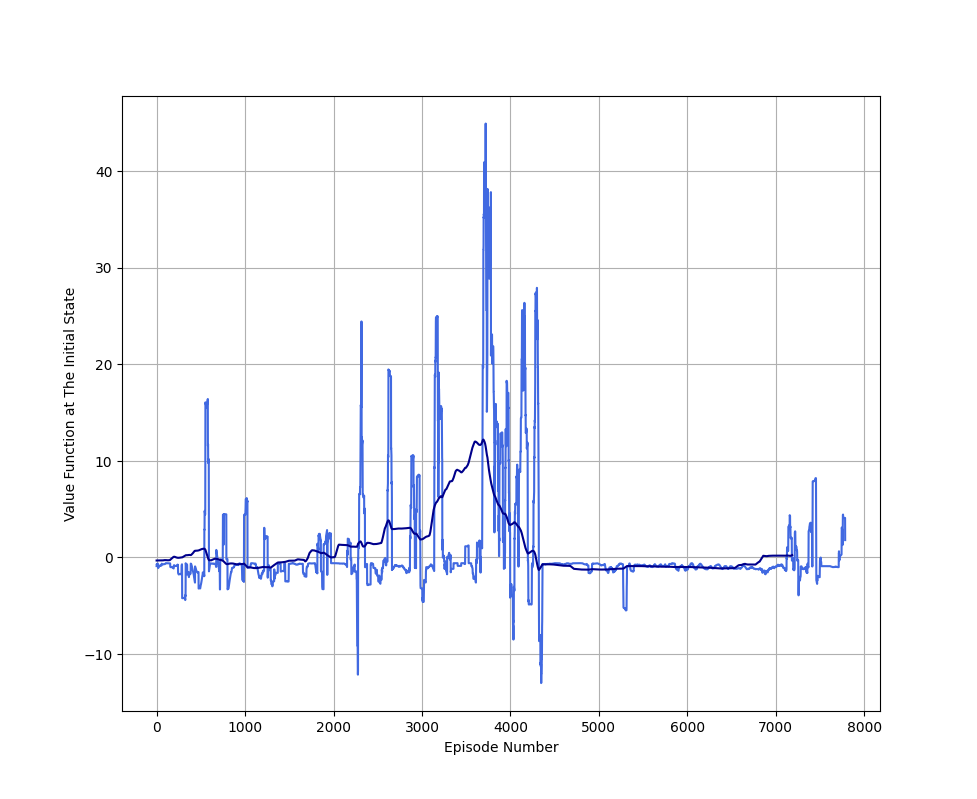
\includegraphics[keepaspectratio,scale=0.5]{media/DDPGValue.png}
    \caption{Value Function of DDPG over Episode Count}
    \label{ddpg}
\end{figure}
\paragraph{Q-Learning}
We began training our agent using Q-learning with hyperparameters set to 20000 episodes, 2000 iterations, discount rate set to 0.95, and a learning rate of 0.05. Q-learning was first trained on a modified version of the track that featured a much wider straight-away to estimate the difficulty of the track. In this wide track, the Q-learning algorithm was successful in finding a reliable route to the goal multiple times within 2000 episodes and achieved roughly 70\% success rate in reaching the goal without violating any of our constraints. However, when switching to the intended narrow track, Q-learning failed to reach the goal a single time over 20,000 episodes. Upon inspection of the environment during training, the agent was hardly able to even make it halfway up the track without running into the side of the wall. We hypothesize this shortcoming to be because as the agent is filling out the Q-Table, due to the sparse reward, it has no bearing on whether it is reaching the goal and is essentially performing random actions until it does. The abstraction process of the environment to a discrete state space also poses trouble for the agent's learning ability as some states may not be represented as well as they should be when discretized.
\paragraph{Neural Fitted Q-Learning}
NFQ was trained using similar hyperparameters as Q-learning, with 20,000 episodes and 2000 iterations and the same discount and learning rate. A memory buffer of 100,000 was set to preserve as much of the Q-Table as possible in the hopes the agent will train faster. The results of testing our agent on the straight-line track using NFQ to learn the environment were unsatisfactory. After roughly 18 hours of training and 20,000 episodes, the agent failed to reach the goal a single time. When observing the agent train, we noticed a common failure that Q-learning performed, which was frequently driving into walls and taking nonsensical pathways to fill out the Q-table. Clearly, the abstraction process of a continuous world such as in CoppeliaSim and reality is a significant hamstring to both Q-learning models. Although we were not able to test NFQ in a wider track to see if it replicated the success Q-Learning had, we have a strong suspicion it would learn similarly, if not faster due to the neural fitting modification to the algorithm.
\paragraph{Deep Deterministic Policy Gradient}
DDPG was trained using the same hyperparameters as the previous two algorithms, along with a similar memory buffer of 100,000 which was left default. However, due to time constraints, the agent's training was restricted to about 8000 episodes. The results of training a DDPG agent on the narrow track were extremely successful. Although a convergence of the value function did not occur which would signify optimal training as seen in \ref{ddpg}, the tested agent achieved a goal success rate of 76\%, meaning the agent is able to reach the goal without violating any of our constraints 76\% of the time. We suspect this success is tied to two factors: the algorithm's ability to handle continuous state spaces and not relying on a Q-Table that must be filled out to find a result. Due to DDPG's specialty in handling continuous state spaces, we were able to remove our rounding actions that discarded information that may have been useful to the Q-Learning algorithms discussed prior. Through visual observation of the agent, we noticed a few intriguing developments of how the agent learns its strategy. At first, the agent would careen into the walls early on the track, but as more episodes occurred, the agent learned to drive straight to put off its failures. However, this strategy is not optimal as the agent must refrain from entering the goal when the traffic light is in the red state. The agent, over time, learned to perform wait actions in between its movements so as to delay its arrival to the goal before the light turned red. We believe given much more training time to allow for value function convergence this agent will master the environment with an extremely high success rate.
\section{Conclusion}
%You still need to conclude something for the midterm
The problems reinforcement learning is well suited for problems which are difficult to solve analytically. Analytical assurances are a major goal of any safety critical system. Logically constrained reinforcement learning can provide some assurances of adherence to some specified logical criteria. However, it is no panacea.

%We need to talk about the limitations and the problems we encountered with training time, learning, and the sparse reward mechanism. Comparing the LDBA based reward shaping with more incremental reward systems.
In our experiences here we can see a clear trade off between the assurances LCRL provides and the sparse reward structure that it entails. Our experiments here show that while our agent did not learn and converge on some less than ideal policy, instead it sometimes did not converge on an ideal policy at all. There is a trade off that is made. Since our best policy did not get higher than 76\% we cannot be assured that our policy will be safe. This also means we know to what degree our policy does not adhere to the logical controls we put forward. More work in reward shaping, increasing training time, and further altering input and state space parameters and algorithm hyperparameters may improve our agent in the future. LCRL is no universal solution, it does not provide a simple answer to all of reinforcement learning's problems, but it does provide some assurance that if a particular policy is found we can know within some statistical certainty that it fulfils all the criteria we require.


\printbibliography %Prints bibliography

\end{document}